\documentclass{standalone}
\usepackage{tikz}
\usetikzlibrary{patterns, positioning}
\usepackage[sfdefault]{ClearSans} %% option 'sfdefault' activates Clear Sans as the default text font
\usepackage[T1]{fontenc}

\begin{document}
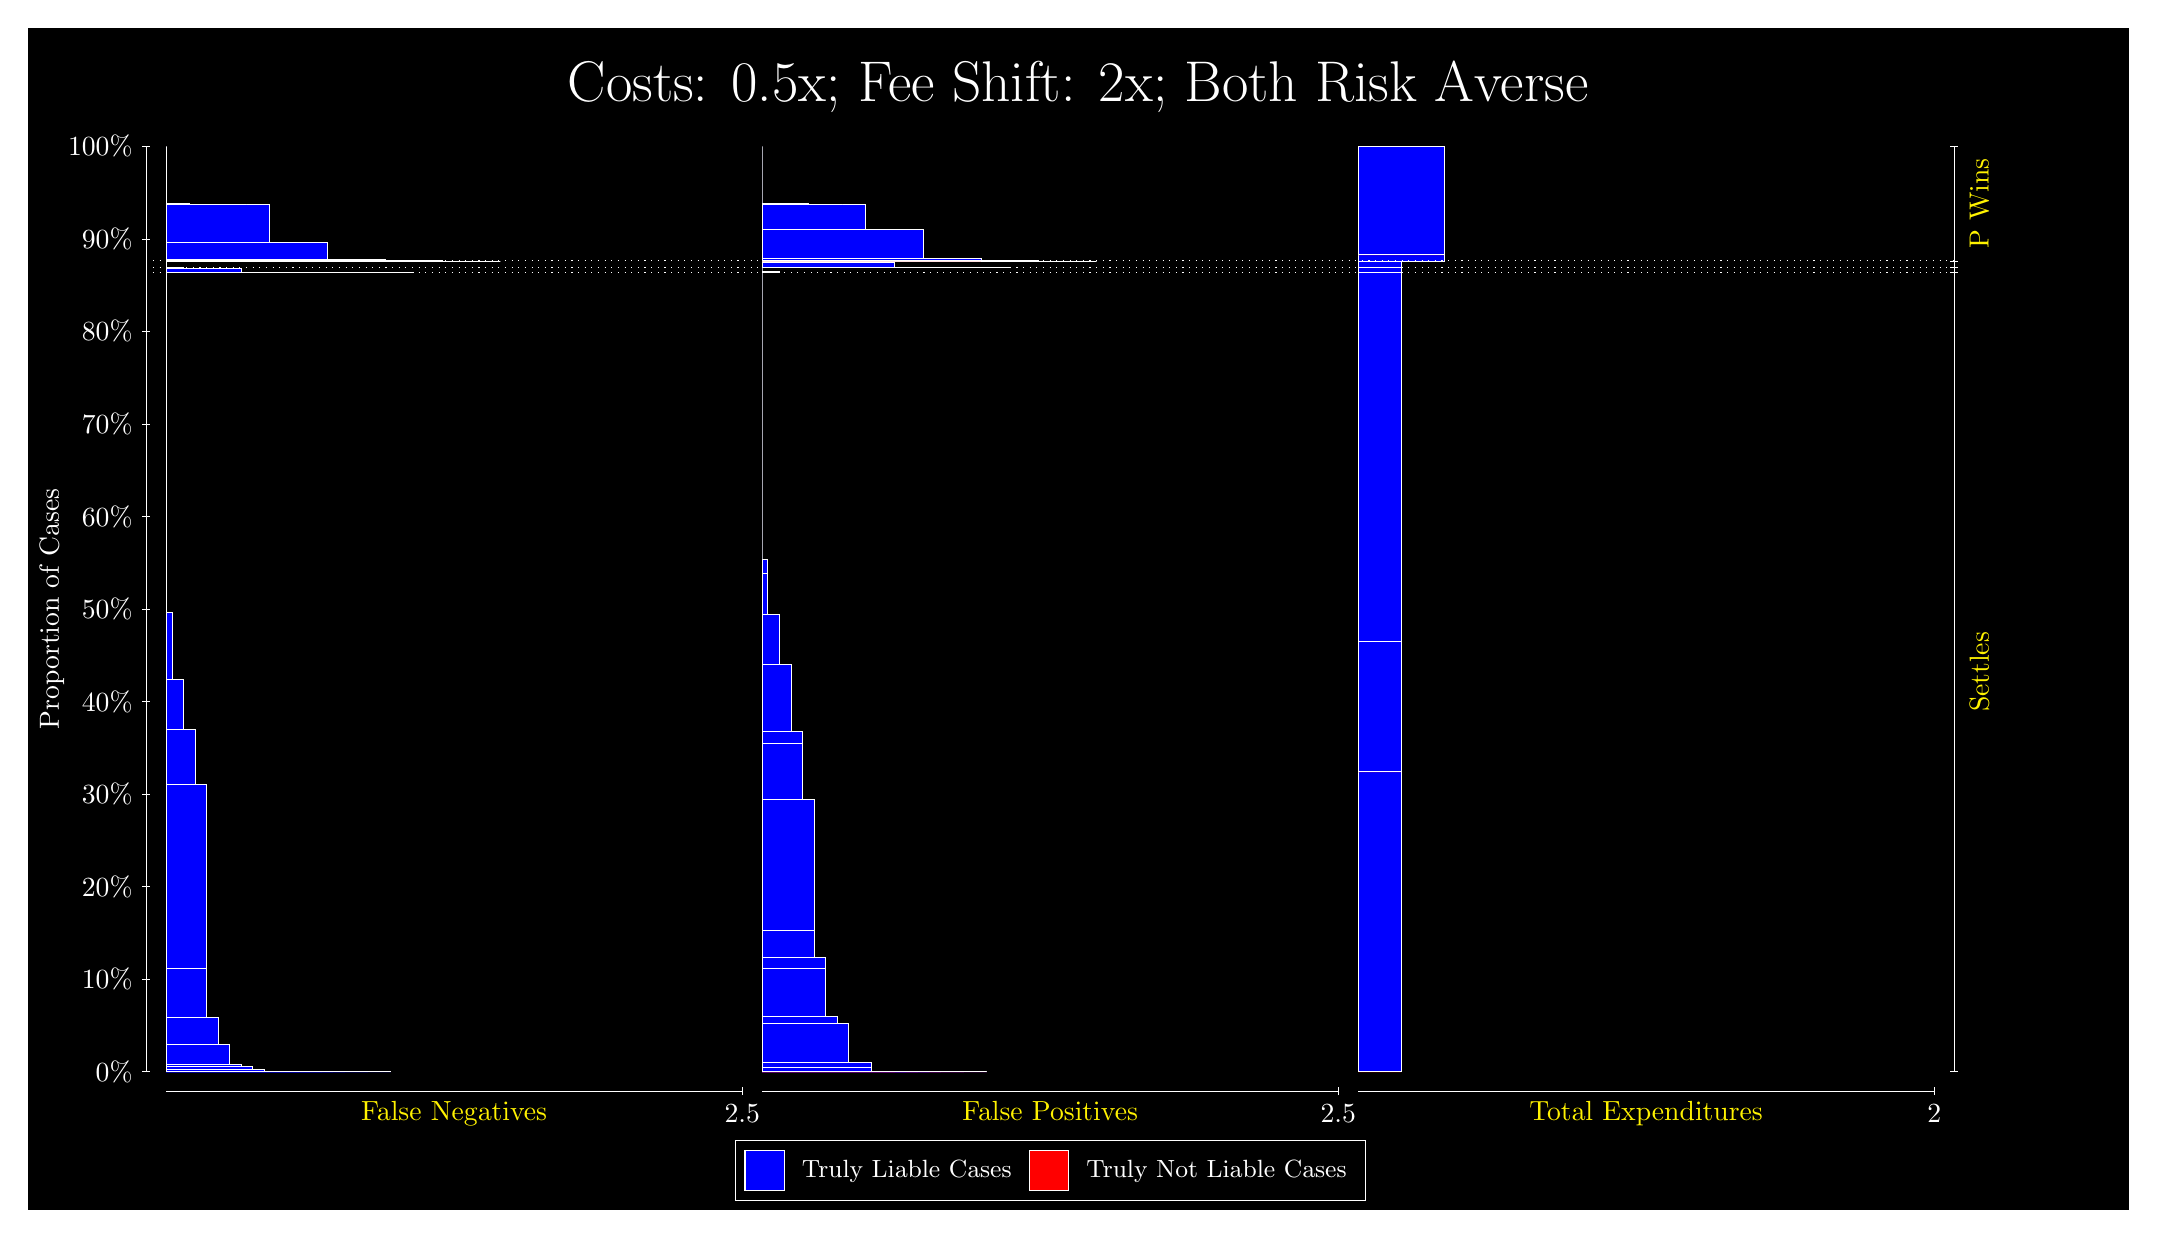
\begin{tikzpicture}
\draw[fill=black] (0,0) rectangle (26.667,15);
\draw[text=white] (0,13.5) rectangle (26.667,15) node[midway] {\huge Costs: 0.5x; Fee Shift: 2x; Both Risk Averse};
\draw[white, very thin] (1.5,1.75) -- (1.5,13.5);
\node[rotate=90, text=white, anchor=center] at (0.3, 7.625) {Proportion of Cases};
\draw[white, very thin] (1.45,1.75) -- (1.55,1.75);
\node[text=white, anchor=east] at (1.45, 1.75) {0\%};
\draw[white, very thin] (1.45,2.925) -- (1.55,2.925);
\node[text=white, anchor=east] at (1.45, 2.925) {10\%};
\draw[white, very thin] (1.45,4.1) -- (1.55,4.1);
\node[text=white, anchor=east] at (1.45, 4.1) {20\%};
\draw[white, very thin] (1.45,5.275) -- (1.55,5.275);
\node[text=white, anchor=east] at (1.45, 5.275) {30\%};
\draw[white, very thin] (1.45,6.45) -- (1.55,6.45);
\node[text=white, anchor=east] at (1.45, 6.45) {40\%};
\draw[white, very thin] (1.45,7.625) -- (1.55,7.625);
\node[text=white, anchor=east] at (1.45, 7.625) {50\%};
\draw[white, very thin] (1.45,8.8) -- (1.55,8.8);
\node[text=white, anchor=east] at (1.45, 8.8) {60\%};
\draw[white, very thin] (1.45,9.975) -- (1.55,9.975);
\node[text=white, anchor=east] at (1.45, 9.975) {70\%};
\draw[white, very thin] (1.45,11.15) -- (1.55,11.15);
\node[text=white, anchor=east] at (1.45, 11.15) {80\%};
\draw[white, very thin] (1.45,12.325) -- (1.55,12.325);
\node[text=white, anchor=east] at (1.45, 12.325) {90\%};
\draw[white, very thin] (1.45,13.5) -- (1.55,13.5);
\node[text=white, anchor=east] at (1.45, 13.5) {100\%};

\draw[white, very thin] (24.457,1.75) -- (24.457,13.5);
\draw[white, very thin] (24.407,1.75) -- (24.507,1.75);
\node[anchor=west] at (24.407, 1.75) {};
\draw[white, very thin] (24.407,11.901) -- (24.507,11.901);
\node[anchor=west] at (24.407, 11.901) {};
\draw[white, very thin] (24.407,11.965) -- (24.507,11.965);
\node[anchor=west] at (24.407, 11.965) {};
\draw[white, very thin] (24.407,12.046) -- (24.507,12.046);
\node[anchor=west] at (24.407, 12.046) {};
\draw[white, very thin] (24.407,13.5) -- (24.507,13.5);
\node[anchor=west] at (24.407, 13.5) {};

\draw[white, very thin, fill=blue] (1.75,1.75) rectangle (4.6044,1.75);
\draw[white, very thin, fill=blue] (1.75,1.75) rectangle (4.3116,1.75);
\draw[white, very thin, fill=blue] (1.75,1.75) rectangle (4.0188,1.75);
\draw[white, very thin, fill=blue] (1.75,1.75) rectangle (3.8725,1.75);
\draw[white, very thin, fill=blue] (1.75,1.75) rectangle (3.7261,1.75);
\draw[white, very thin, fill=blue] (1.75,1.75) rectangle (3.5797,1.75);
\draw[white, very thin, fill=blue] (1.75,1.75) rectangle (3.4333,1.75);
\draw[white, very thin, fill=blue] (1.75,1.75) rectangle (3.287,1.7517);
\draw[white, very thin, fill=blue] (1.75,1.7517) rectangle (3.1406,1.7585);
\draw[white, very thin, fill=blue] (1.75,1.7585) rectangle (2.9942,1.7585);
\draw[white, very thin, fill=blue] (1.75,1.7585) rectangle (2.9942,1.7842);
\draw[white, very thin, fill=blue] (1.75,1.7842) rectangle (2.8478,1.8124);
\draw[white, very thin, fill=blue] (1.75,1.8124) rectangle (2.7015,1.843);
\draw[white, very thin, fill=blue] (1.75,1.843) rectangle (2.5551,2.0993);
\draw[white, very thin, fill=blue] (1.75,2.0993) rectangle (2.5551,2.0993);
\draw[white, very thin, fill=blue] (1.75,2.0993) rectangle (2.4087,2.4423);
\draw[white, very thin, fill=blue] (1.75,2.4423) rectangle (2.2623,2.4435);
\draw[white, very thin, fill=blue] (1.75,2.4435) rectangle (2.2623,3.0592);
\draw[white, very thin, fill=blue] (1.75,3.0592) rectangle (2.2623,5.4016);
\draw[white, very thin, fill=blue] (1.75,5.4016) rectangle (2.1159,6.0969);
\draw[white, very thin, fill=blue] (1.75,6.0969) rectangle (1.9696,6.7261);
\draw[white, very thin, fill=blue] (1.75,6.7261) rectangle (1.8232,7.5813);
\draw[white, very thin, fill=blue] (1.75,7.5813) rectangle (1.8232,7.5813);
\draw[white, very thin, fill=red] (1.75,7.5813) rectangle (1.75,7.5813);
\draw[white, very thin, fill=blue] (1.75,7.5813) rectangle (1.75,11.901);
\draw[white, very thin, fill=blue] (1.75,11.901) rectangle (4.8971,11.901);
\draw[white, very thin, fill=blue] (1.75,11.901) rectangle (4.1652,11.901);
\draw[white, very thin, fill=blue] (1.75,11.901) rectangle (3.4333,11.905);
\draw[white, very thin, fill=blue] (1.75,11.905) rectangle (2.7015,11.948);
\draw[white, very thin, fill=blue] (1.75,11.948) rectangle (1.9696,11.965);
\draw[white, very thin, fill=red] (1.75,11.965) rectangle (1.75,11.965);
\draw[white, very thin, fill=blue] (1.75,11.965) rectangle (1.9696,11.965);
\draw[white, very thin, fill=red] (1.75,11.965) rectangle (1.75,11.965);
\draw[white, very thin, fill=blue] (1.75,11.965) rectangle (1.75,12.046);
\draw[white, very thin, fill=blue] (1.75,12.046) rectangle (5.9949,12.046);
\draw[white, very thin, fill=blue] (1.75,12.046) rectangle (5.2631,12.047);
\draw[white, very thin, fill=blue] (1.75,12.047) rectangle (4.5312,12.062);
\draw[white, very thin, fill=blue] (1.75,12.062) rectangle (3.7993,12.28);
\draw[white, very thin, fill=blue] (1.75,12.28) rectangle (3.5065,12.28);
\draw[white, very thin, fill=blue] (1.75,12.28) rectangle (3.0674,12.767);
\draw[white, very thin, fill=blue] (1.75,12.767) rectangle (2.7746,12.767);
\draw[white, very thin, fill=blue] (1.75,12.767) rectangle (2.3355,12.767);
\draw[white, very thin, fill=blue] (1.75,12.767) rectangle (2.0428,12.777);
\draw[white, very thin, fill=red] (1.75,12.777) rectangle (1.75,12.777);
\draw[white, very thin, fill=blue] (1.75,12.777) rectangle (1.75,13.5);
\draw[white, very thin, fill=red] (9.3189,1.75) rectangle (12.173,1.75);
\draw[white, very thin, fill=blue] (9.3189,1.75) rectangle (12.173,1.75);
\draw[white, very thin, fill=red] (9.3189,1.75) rectangle (11.88,1.75);
\draw[white, very thin, fill=blue] (9.3189,1.75) rectangle (11.88,1.75);
\draw[white, very thin, fill=red] (9.3189,1.75) rectangle (11.588,1.75);
\draw[white, very thin, fill=blue] (9.3189,1.75) rectangle (11.588,1.75);
\draw[white, very thin, fill=blue] (9.3189,1.75) rectangle (11.441,1.75);
\draw[white, very thin, fill=red] (9.3189,1.75) rectangle (11.295,1.75);
\draw[white, very thin, fill=blue] (9.3189,1.75) rectangle (11.295,1.75);
\draw[white, very thin, fill=blue] (9.3189,1.75) rectangle (11.149,1.7501);
\draw[white, very thin, fill=red] (9.3189,1.7501) rectangle (11.002,1.7501);
\draw[white, very thin, fill=blue] (9.3189,1.7501) rectangle (11.002,1.7509);
\draw[white, very thin, fill=blue] (9.3189,1.7509) rectangle (10.856,1.7515);
\draw[white, very thin, fill=red] (9.3189,1.7515) rectangle (10.709,1.7515);
\draw[white, very thin, fill=blue] (9.3189,1.7515) rectangle (10.709,1.8083);
\draw[white, very thin, fill=red] (9.3189,1.8083) rectangle (10.709,1.8083);
\draw[white, very thin, fill=blue] (9.3189,1.8083) rectangle (10.709,1.8699);
\draw[white, very thin, fill=blue] (9.3189,1.8699) rectangle (10.563,1.8727);
\draw[white, very thin, fill=red] (9.3189,1.8727) rectangle (10.417,1.8727);
\draw[white, very thin, fill=blue] (9.3189,1.8727) rectangle (10.417,2.3622);
\draw[white, very thin, fill=blue] (9.3189,2.3622) rectangle (10.27,2.4524);
\draw[white, very thin, fill=red] (9.3189,2.4524) rectangle (10.124,2.4524);
\draw[white, very thin, fill=blue] (9.3189,2.4524) rectangle (10.124,3.0558);
\draw[white, very thin, fill=blue] (9.3189,3.0558) rectangle (10.124,3.1971);
\draw[white, very thin, fill=blue] (9.3189,3.1971) rectangle (9.9776,3.5419);
\draw[white, very thin, fill=blue] (9.3189,3.5419) rectangle (9.9776,5.2086);
\draw[white, very thin, fill=red] (9.3189,5.2086) rectangle (9.8312,5.2086);
\draw[white, very thin, fill=blue] (9.3189,5.2086) rectangle (9.8312,5.917);
\draw[white, very thin, fill=blue] (9.3189,5.917) rectangle (9.8312,6.0696);
\draw[white, very thin, fill=blue] (9.3189,6.0696) rectangle (9.6848,6.9248);
\draw[white, very thin, fill=blue] (9.3189,6.9248) rectangle (9.5384,7.5539);
\draw[white, very thin, fill=blue] (9.3189,7.5539) rectangle (9.3921,8.0838);
\draw[white, very thin, fill=blue] (9.3189,8.0838) rectangle (9.3921,8.2492);
\draw[white, very thin, fill=blue] (9.3189,8.2492) rectangle (9.3189,11.901);
\draw[white, very thin, fill=red] (9.3189,11.901) rectangle (9.5384,11.901);
\draw[white, very thin, fill=blue] (9.3189,11.901) rectangle (9.5384,11.918);
\draw[white, very thin, fill=blue] (9.3189,11.918) rectangle (9.3189,11.965);
\draw[white, very thin, fill=red] (9.3189,11.965) rectangle (12.466,11.965);
\draw[white, very thin, fill=blue] (9.3189,11.965) rectangle (12.466,11.965);
\draw[white, very thin, fill=blue] (9.3189,11.965) rectangle (11.734,11.968);
\draw[white, very thin, fill=blue] (9.3189,11.968) rectangle (11.002,12.022);
\draw[white, very thin, fill=blue] (9.3189,12.022) rectangle (10.27,12.046);
\draw[white, very thin, fill=blue] (9.3189,12.046) rectangle (9.5384,12.046);
\draw[white, very thin, fill=red] (9.3189,12.046) rectangle (13.564,12.046);
\draw[white, very thin, fill=blue] (9.3189,12.046) rectangle (13.564,12.046);
\draw[white, very thin, fill=red] (9.3189,12.046) rectangle (12.832,12.046);
\draw[white, very thin, fill=blue] (9.3189,12.046) rectangle (12.832,12.047);
\draw[white, very thin, fill=red] (9.3189,12.047) rectangle (12.1,12.047);
\draw[white, very thin, fill=blue] (9.3189,12.047) rectangle (12.1,12.077);
\draw[white, very thin, fill=red] (9.3189,12.077) rectangle (11.368,12.077);
\draw[white, very thin, fill=blue] (9.3189,12.077) rectangle (11.368,12.449);
\draw[white, very thin, fill=blue] (9.3189,12.449) rectangle (10.636,12.769);
\draw[white, very thin, fill=red] (9.3189,12.769) rectangle (10.344,12.769);
\draw[white, very thin, fill=blue] (9.3189,12.769) rectangle (10.344,12.769);
\draw[white, very thin, fill=blue] (9.3189,12.769) rectangle (9.9044,12.779);
\draw[white, very thin, fill=red] (9.3189,12.779) rectangle (9.6116,12.779);
\draw[white, very thin, fill=blue] (9.3189,12.779) rectangle (9.6116,12.78);
\draw[white, very thin, fill=blue] (9.3189,12.78) rectangle (9.6116,12.78);
\draw[white, very thin, fill=red] (9.3189,12.78) rectangle (9.3189,12.78);
\draw[white, very thin, fill=blue] (9.3189,12.78) rectangle (9.3189,13.5);
\draw[white, very thin, fill=red] (16.888,1.75) rectangle (17.437,1.75);
\draw[white, very thin, fill=blue] (16.888,1.75) rectangle (17.437,5.5575);
\draw[white, very thin, fill=red] (16.888,5.5575) rectangle (17.437,5.5575);
\draw[white, very thin, fill=blue] (16.888,5.5575) rectangle (17.437,7.217);
\draw[white, very thin, fill=red] (16.888,7.217) rectangle (17.437,7.217);
\draw[white, very thin, fill=blue] (16.888,7.217) rectangle (17.437,11.901);
\draw[white, very thin, fill=red] (16.888,11.901) rectangle (17.437,11.901);
\draw[white, very thin, fill=blue] (16.888,11.901) rectangle (17.437,11.965);
\draw[white, very thin, fill=red] (16.888,11.965) rectangle (17.437,11.965);
\draw[white, very thin, fill=blue] (16.888,11.965) rectangle (17.437,12.046);
\draw[white, very thin, fill=red] (16.888,12.046) rectangle (17.986,12.046);
\draw[white, very thin, fill=blue] (16.888,12.046) rectangle (17.986,12.126);
\draw[white, very thin, fill=red] (16.888,12.126) rectangle (17.986,12.126);
\draw[white, very thin, fill=blue] (16.888,12.126) rectangle (17.986,13.5);
\draw[white, dotted] (1.5,11.901) -- (24.457,11.901);
\draw[white, dotted] (1.5,11.965) -- (24.457,11.965);
\draw[white, dotted] (1.5,12.046) -- (24.457,12.046);
\draw[white, very thin] (1.75,1.5) -- (9.0689,1.5);
\node[text=yellow, anchor=north] at (5.4094, 1.5) {False Negatives};
\draw[white, very thin] (9.0689,1.45) -- (9.0689,1.55);
\node[text=white, anchor=north] at (9.0689, 1.45) {2.5};

\draw[white, very thin] (9.3189,1.5) -- (16.638,1.5);
\node[text=yellow, anchor=north] at (12.978, 1.5) {False Positives};
\draw[white, very thin] (16.638,1.45) -- (16.638,1.55);
\node[text=white, anchor=north] at (16.638, 1.45) {2.5};

\draw[white, very thin] (16.888,1.5) -- (24.207,1.5);
\node[text=yellow, anchor=north] at (20.547, 1.5) {Total Expenditures};
\draw[white, very thin] (24.207,1.45) -- (24.207,1.55);
\node[text=white, anchor=north] at (24.207, 1.45) {2};

\node[text=yellow, centered, rotate=90] at (24.777, 6.8254) {Settles};


\node[text=yellow, centered, rotate=90] at (24.777, 12.773) {P Wins};

\draw (12.978300999999998,1.5) node[draw=none] (baseCoordinate) {};
\begin{scope}[align=center]
        \matrix[scale=0.5, draw=white, below=0.5cm of baseCoordinate, nodes={draw}, column sep=0.1cm]{
            \node[rectangle, draw, minimum width=0.5cm, minimum height=0.5cm, fill=blue] {}; &
            \node[draw=none, font=\small, text=white] (B) {Truly Liable Cases}; &
            \node[rectangle, draw, minimum width=0.5cm, minimum height=0.5cm, fill=red] {}; &
            \node[draw=none, font=\small, text=white] (B) {Truly Not Liable Cases}; \\
            };
\end{scope}

\end{tikzpicture}
\end{document}